\section{Auxiliary functions}
    In this section, we will present the auxiliary function used in the nodes of our BT algorithm.\\
    These will include the functions used for conversions, more complex or repetitive mathematical operations, and other functions that are not directly related to the BT algorithm.\\
    One of the big sections will be the algorithms used for determining the classification and cost of roads in the road network.\\
    We will split the functions into categories based on their purpose.

    \subsection{Road cost algorithm}
        We will use the algorithm developed during the summer of 2022 for the RobInGas project at the CTU CRAS. The algorithm was designed to determine the cost of crossing the road based on the road classification, curvature, and other factors.\\
        We will briefly present the functionality of the algorithm. The full description with implementation details can be found in \cite{Road_cost_docs}.\\
        This is also the only part of our thesis written in Python instead of \CC\ this is due to it being part of a different project. Other reasons include the usage of libraries for Python. While we could rewrite the code to \CC\ it was not deemed necessary as this part is run only once at the beginning of the mission and therefore does not need to be optimized for speed.\\\\
        \bfc{Overview}\\
            We use multiple parameters to determine the cost of crossing. The most important ones are the geometrical properties of the road. This includes the curvature of the road, the elevation profile, and the proximity to intersections. We also use the road classification to add to the cost function.\\
            Other parameters would be beneficiary, such as the road width, the presence of a pedestrian crossing, and the expected traffic speed.\\
            Unfortunately, we do not have access to all of these parameters. We use the OSM data, which does not necessarily contain all those additional parameters. Therefore, we will inject this information directly into the algorithm and deal with these parameters separately.\\
            The OSM data also do not contain the elevation profile of the road. This data is also not easily obtainable from free or open-source sources. The elevation data we use were purchased from the Land Survey Office of the Czech Republic. We use the ZABAGED\footnote{\url{https://geoportal.cuzk.cz/(S(dcpfei0nmxcwgoe4frurwfgm))/Default.aspx?lng=EN&mode=TextMeta&text=dSady_zabaged&side=zabaged&menu=24}} data. This data from the Land Survey Office are available only for the area of the Czech Republic. However, any file with elevation data with the correct formatting can be used. The used file format is as follows. A text file with the easting, northing, and altitude of one point is on one line separated by a space. The lines are separated with a newline character \texttt{\textbackslash n}, each describing exactly one point.\\
            If the elevation data are not provided, the algorithm will still function. It will just not take the elevation profile into account. The road cost will be determined only from the curvate and road classification.\\\\
        \bfc{Algorithm}\\
            The algorithm is divided into several parts.\\
            The first part is obtaining the road segments from downloaded OSM data. This part is also responsible for logging the road classification for each segment.\\
            The second part is responsible for determining the curvature of the roads. This is done by calculating the radius of the circumcircle of the triangle formed by the two adjacent road segments. This approach is visualized in image \ref{fig:curvature}. We then sort the road segments into multiple classes based on their radius. In this part, we also detect road junctions and penalize the road segments close to the junction.\\
            In the third part, we determine the elevation profile of the road. We then classify the individual road segments with the TPI (Terrain Profile Index) method. Some TPI classes are presented in image \ref{fig:TPI}.\\
            In the last part, we combine the results from the previous parts and calculate the final cost of crossing for each segment.
            \begin{figure}[H]
            \centering
            \begin{subfigure}[b]{0.45\textwidth}
                \centering
                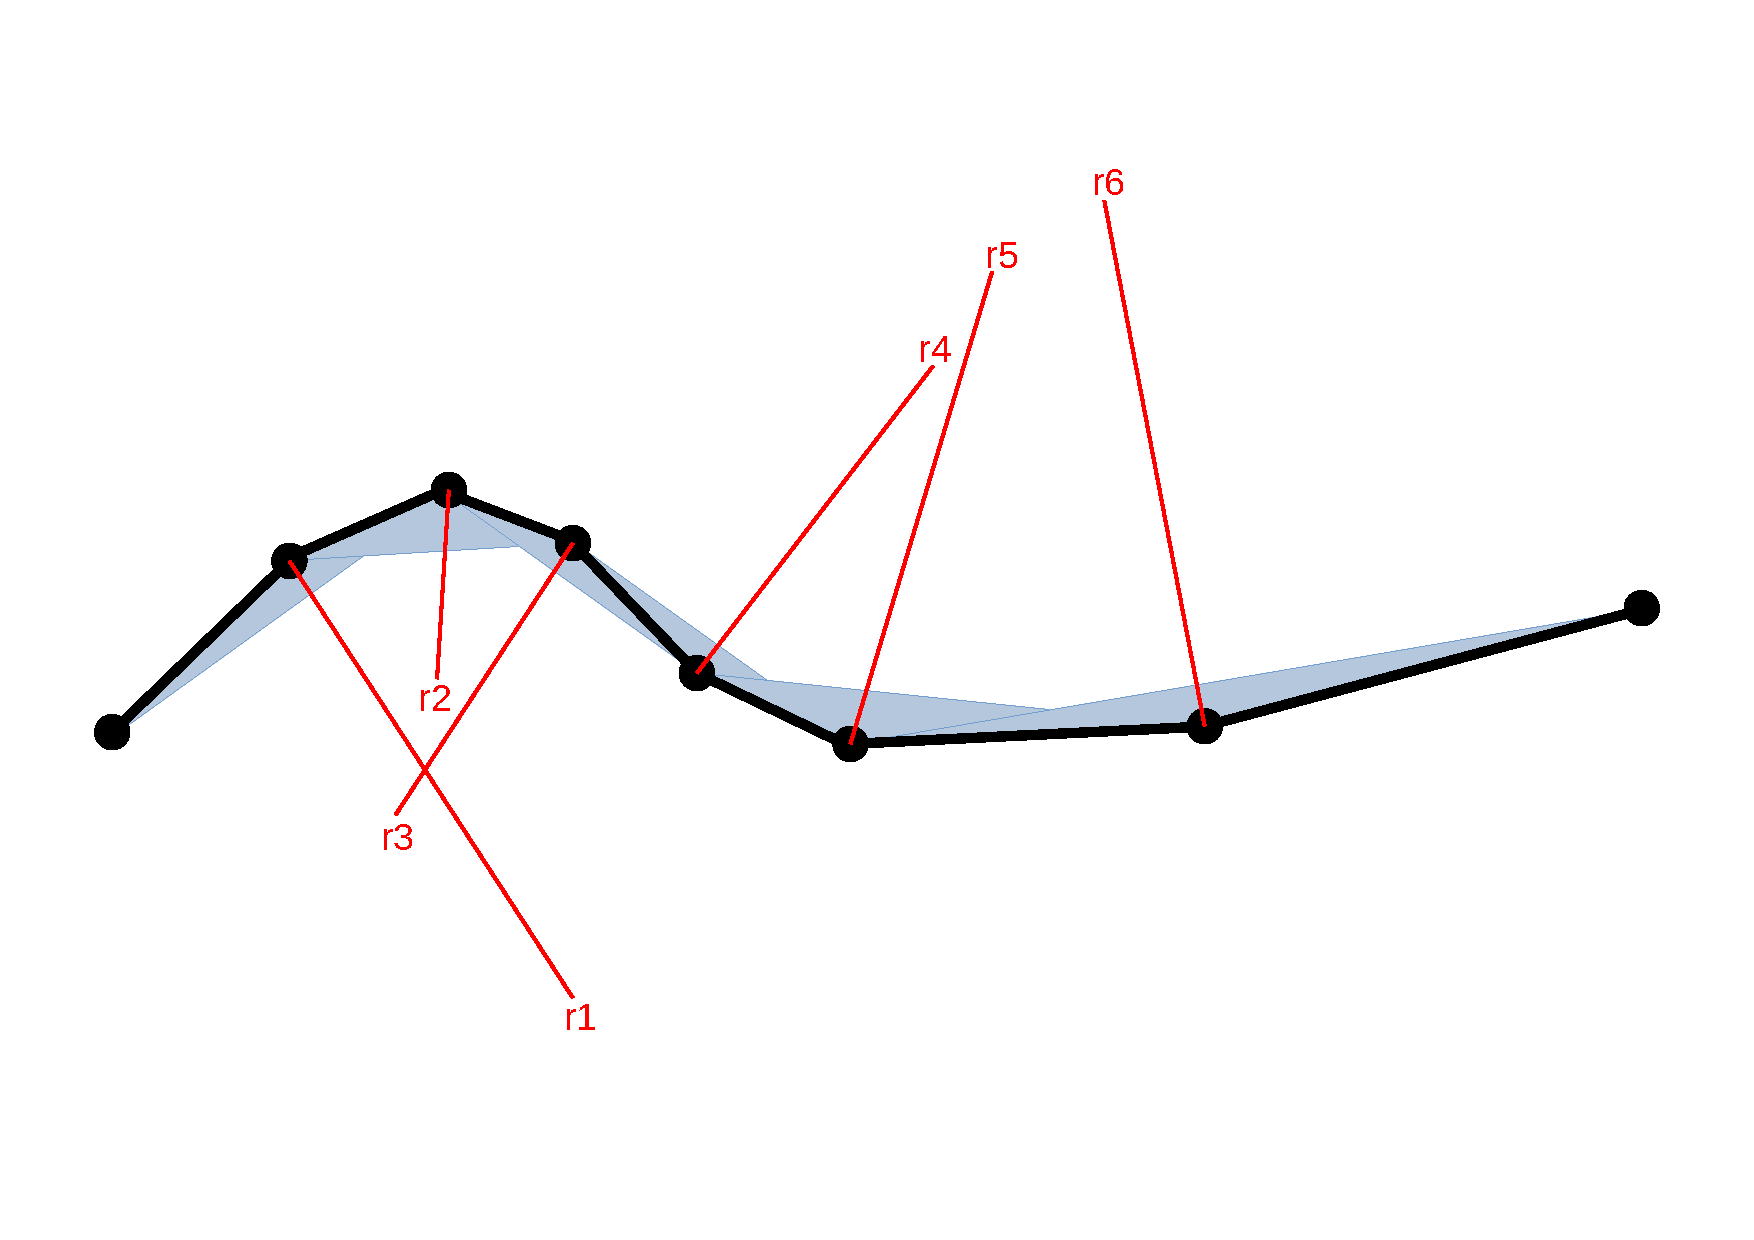
\includegraphics[width=\textwidth]{images/path_curvature.pdf}
                \caption{Visualization of the circumcircle radii.}
                \label{fig:curvature}
            \end{subfigure}
            \begin{subfigure}[b]{0.45\textwidth}
                \centering
                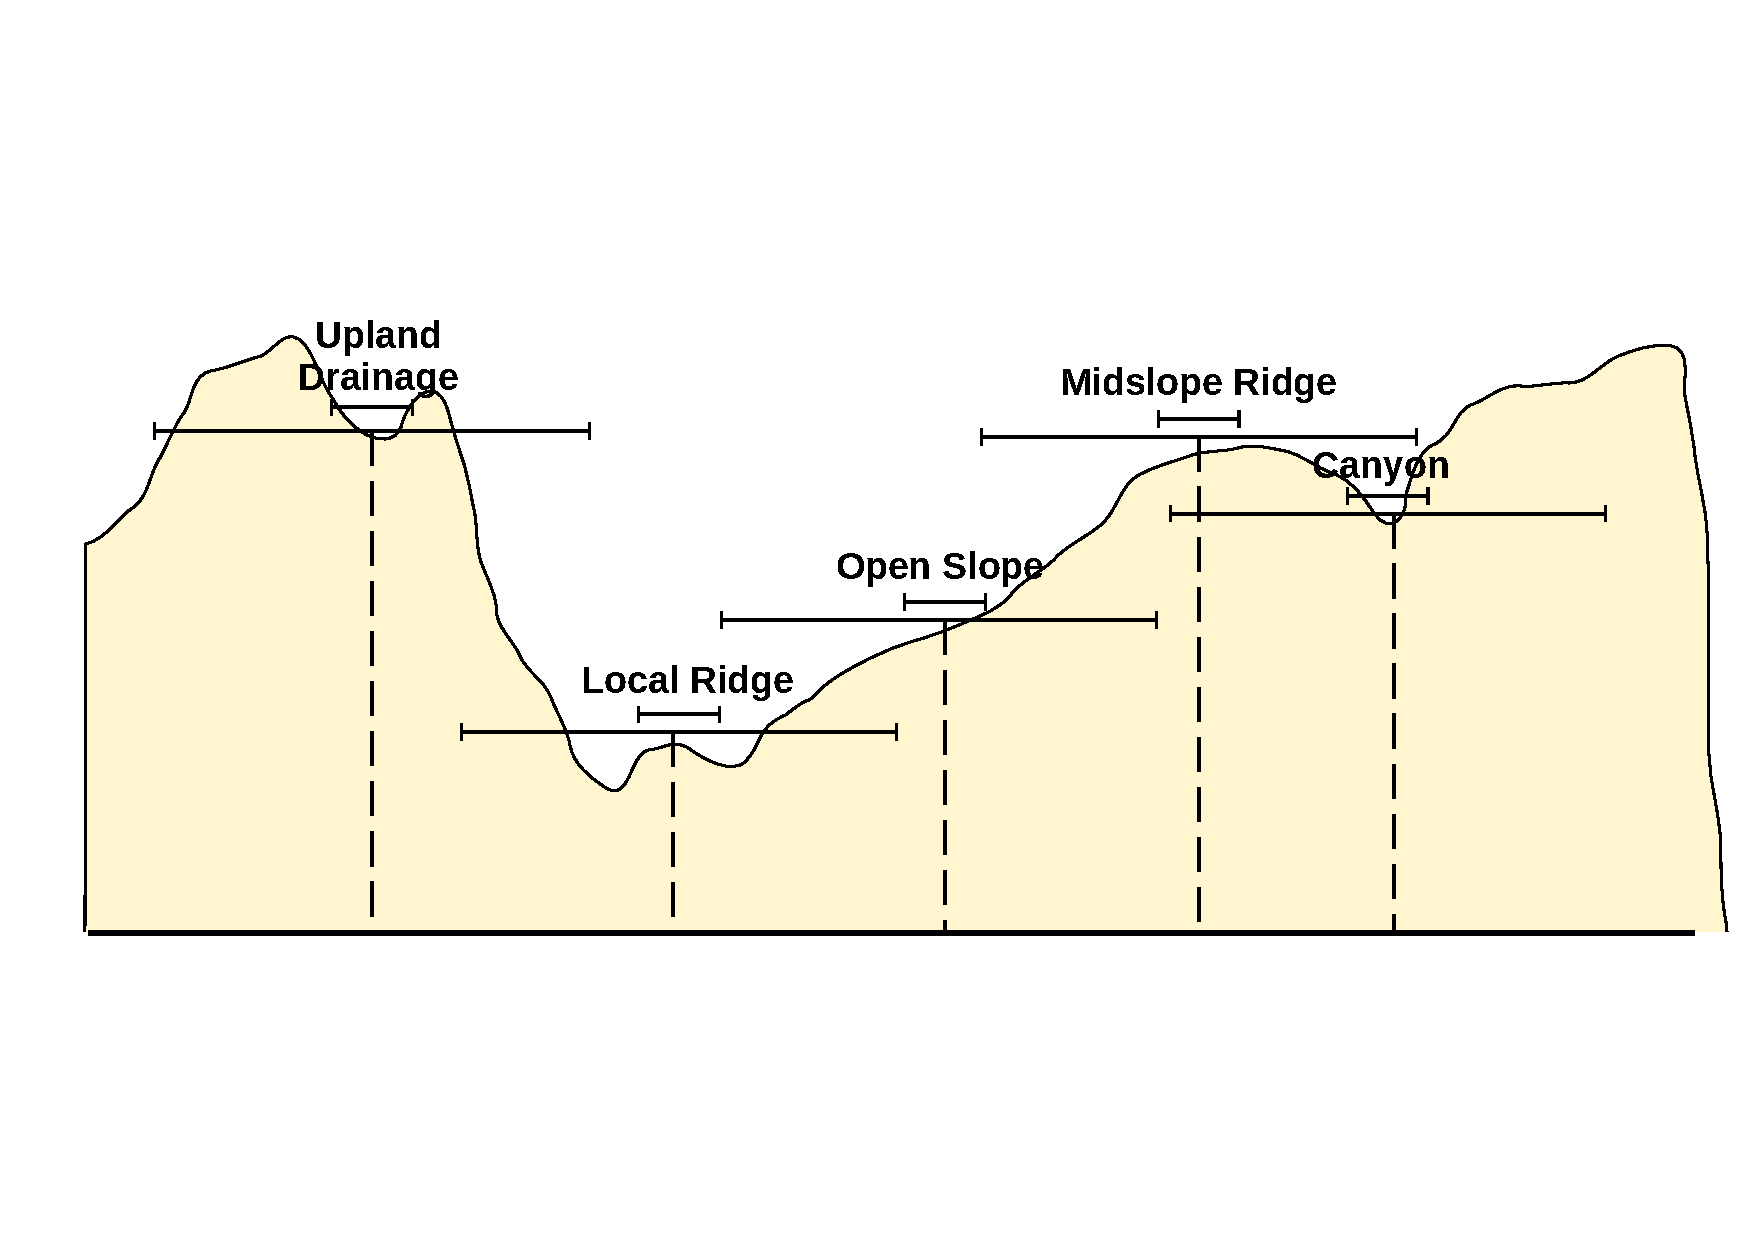
\includegraphics[width=\textwidth]{images/TPI_classification.pdf}
                \caption{Representation of certain TPI classes.}
                \label{fig:TPI}
            \end{subfigure}
            \caption{Visualization of key elements in road cost algorithm.}
        \end{figure}

        \bfc{Usage}\\
            As was stated earlier, this algorithm is executed only once at the beginning of the mission. Later we only keep the final costs, and based on them, we determine if the location where the robot is trying to cross is suitable and safe.\\
            We rely on ROS to enable the communication between our main algorithm and the algorithm for determining the suitability of the location for crossing. We use the ROS service for this purpose.\\
            Another part of the algorithm is to try and provide the robot with a more suitable place for crossing if the current location is unsuitable. If such a place is found and provided we will publish a cost map that will be used to change the current cost map of the path planner. This is done so that we do not need to override the robot's controls until we begin the crossing itself.

    \subsection{Mathematical functions}
        \bfc{Difference between two angles}\\
            This function is used to determine the difference between two given angles. We assume the angles given are in radians, and both are in the interval $\langle0;2\pi\rangle$. This difference is calculated to be the smallest possible and to fit within the interval $\langle-\pi;\pi\rangle$. The formula we use is a modified version of the one provided here \cite{calc_rotation}. The formula is as follows
            \begin{equation}
                \Delta\varphi = \left((\varphi_{2} - \varphi_{1} + \pi) \mod (2\pi)\right) - \pi.
            \end{equation}
            Before returning the result, we check whether the result is within the specified interval.\\\\
        \bfc{Converting degrees to radians}\\
            While this function is elementary in its nature, it is often used in our code. Therefore it is beneficiary to create this function.\\
            The equation for converting degrees to radians which this function uses, is as follows
            \begin{equation}
                \varphi_{\rm{RAD}} = \varphi_{\rm{DEG}}\:\frac{\pi}{180}.
            \end{equation}

    \subsection{Geographical functions}
    \label{sec:geo_func}
        Here we will present the functions used for geographical calculations. These include conversions between coordinate systems, calculating azimuths, and others.\\\\
        \bfc{Converting GPS to UTM}\\
            While most geographical data are stored in the WGS84 coordinate system, the UTM coordinate system is more suitable for calculations. We, therefore, need to convert the GPS coordinates to UTM.\\
            We use the GeographicLib library for this purpose. The function from this library that we use is \texttt{GeographicLib::UTMUPS::Forward}. This function takes the point's latitude and longitude and returns the point's easting and northing in the UTM coordinate system. It also returns the zone number and whether the point is in the northern or southern hemisphere.\\
            While the input variables are passed by value, the return variables are passed to the function call by reference.\\\\
        \bfc{Converting NED to ENU}\\
            There are two possible orientations of an azimuth. The NED (North-East-Down) and the ENU (East-North-Up).\\
            NED means that azimuth 0 points north, and its value increases clockwise. This orientation is mainly used in cartography and everyday life.\\
            ENU means that azimuth 0 points east, and its value increases clockwise. This orientation is mainly used in navigation and robotics, as it is consistent with REP-103.\\
            In the entire project, we use the ENU orientation. However, as we rely on other ROS nodes to provide us with the azimuth, we need to be able to convert the azimuth from NED to ENU.\\
            The conversion should be much simpler since we do not deal with coordinates but with already computed azimuths.\\
            The image \ref{fig:dir_indi} shows the two possible orientations of the azimuth. This image also provides us with the insight we need to determine the conversion formula. We need to divide the formula into two parts.
            \begin{figure}[H]
                \centering
                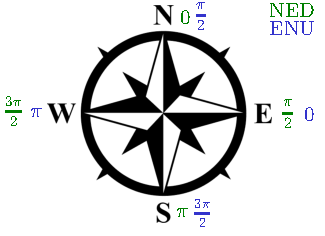
\includegraphics[width=0.5\textwidth]{images/direction_indicator.pdf}
                \caption{Two possible orientations of the azimuth.}
                \label{fig:dir_indi}
            \end{figure}
            \noindent The first option is when the azimuth (in NED) is between 0 and $\frac{\pi}{2}$ rad. In this case, the azimuth in ENU is computed in the following way
            \begin{equation}
                a_{\rm{ENU}} = \frac{\pi}{2} - a_{\rm{NED}},
            \end{equation}
            where $\text{a}_{\rm{ENU}}$ is the azimuth in ENU and $\text{a}_{\rm{NED}}$ is the azimuth in NED.\\
            The second option is for all other azimuths, e.g., when the azimuth is between $\frac{\pi}{2}$ and $2\pi$ rad. In this case, the azimuth in ENU is computed in the following way
            \begin{equation}
                a_{\rm{ENU}} = \frac{5\pi}{2} - a_{\rm{NED}}.
            \end{equation}\\\\
        \bfc{Compute azimuth from coordinates}\\
            This function is used to compute the azimuth for an observer standing at the first point and looking at the second point.\\
            We will use a slightly modified version of the formula provided here \cite{calc_bearing}. This calculation was created for the WGS84 coordinate system, however, we use the UTM coordinate system. Having said that, we can use the same formula, as the WGS84 to UTM projection is conformal\cite{Map_projections}.\\\\
        \bfc{Compute heading for robot}\\
            The use of this function is to determine the heading of the robot. It is used to get the robot perpendicular to the road.\\
            The function takes the robot's heading and the road's azimuth. The road azimuth was obtained using the function stated above.\\
            The algorithm creates two new variables, one $+\pi$ and one $-\pi$ from the road's azimuth. This is necessary as we do not know in what order are road points stored and we do not need to differentiate the side we approach the road from.\\
            Then it computes the difference between the robot's heading and the two new azimuths. The smallest difference is then returned.\\\\
